
Dieser Versuch befasst sich mit der an einer Diode, einem nichtlinearem Bauteil, gemessenen Momentanleistung. Es wird kurz auf den Zusammenhang zwischen Strom, Spannung und Momentanleistung eingegangen, und eine vereinfachte Fourier-Transformation wird durchgeführt.

\subsubsection{Versuchsaufbau}
Der Versuchsaufbau ähnelt weitestgehend dem in Abschnitt \ref{sec:Aufbau2.2.1} beschriebenen. Die Verbraucher werden jedoch ersetzt durch eine Diode sowie einem Vorwiderstand von $R_V=50\Omega$. $u_I(t)$ und $u_U$ werden weiterhin im Oszilloskop zu einer zu $p(t)$ proportionalen Kurve multipliziert.
$R_I$ wird so eingestellt, dass das Spannungsmessgerät $u_{ges} = u_{max} = 9V$ anzeigt.

\subsubsection{Auswertung der Momentanleistungskurve}

Wie in Abschnitt \ref{sec:Versuch2.2.1} erläutert wird die Momentanleistungskurve mit dem Oszilloskop aufgenommen. Sie ist in Abbildung \ref{fig:MomLKurveNichtlinear} zu sehen. $u_U(t)$ ist in Rot, $u_I(t)$ in Blau und das zu $p(t)$ proportionale Produkt der Spannungen ist in Grün zu sehen.

\begin{figure}[H]
\centering
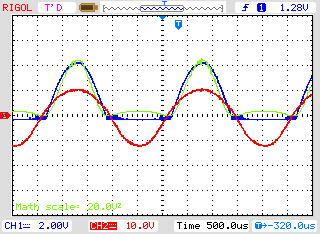
\includegraphics[width=0.8\linewidth]{Oszi-Bitmaps/NewFile5.jpg}
\caption{Momentanleistung einer nichtlinearen Belastung. $u_I(t)$ (Blau), $u_{Z_{ges}}(t)$ (Rot), $p_(t)$ (Grün)}
\label{fig:MomLKurveNichtlinear}
\end{figure}

Deutlich zu sehen ist die nichtlineare Eigenschaft der Diode. In einer Hälfte der Spannungskurve leitet die Diode, die Spannung fällt über dem Widerstand ab und es wird Wirkleistung umgesetzt. In der nächsten Hälfte wird die Diode in Sperrichtung betrieben, es fließt bis auf einen kleinen Leckstrom kein Strom mehr, und es wird keine Leistung mehr umgesetzt.
Zu sehen ist auch, dass die Diode sich nicht wie eine komplexe Impedanz verhält. Strom und Spannung sind nicht phasenverschoben und die Kurve der Momentanleistung ist ausschließlich positiv, von der Schaltung wird nie Leistung abgegeben. Zu bemerken ist auch, dass die Momentanleistung nun die gleiche Frequenz wie die Erregerfrequenz besitzt.

Eine erste Abschätzung der umgesetzten Leistung ergibt sich zu:
\begin{equation*}
P = \frac{1}{2} UI = \frac{1}{4}\hat{U}\hat{I}
\end{equation*}
Grund dafür ist, dass sich die Schaltung für eine halbe Periode wie ein ohm'scher Verbraucher verhält, die nächste halbe Periode jedoch wie ein offener Schaltkreis.

Zur Vereinfachung der Fourier-Analyse wird angenommen, dass die Funktion des Stromes wie folgt definiert ist:
\begin{equation}
i(t)=\hat{I}\cdot \left\{ 
\begin{array}{ccr}
	sin(\omega t) & \mbox{for} & kT < t \leq (k+\frac{1}{2})T \\
	0 & \mbox{for} & (k+\frac{1}{2})T < t \leq (k+1)T
\end{array}
\right.
\end{equation}
\cite{calpolyFourier}

Anhand eines Tabellenbuches für Fourier-Transformationen lässt sich ablesen, dass sich $i(t)$ mit folgender Reihe annähern lässt:
\begin{equation}
i(t) = \frac{\hat{I}}{\pi} + \frac{\hat{I}}{2}\sin(\omega t) - \frac{2\hat{I}}{\pi}\sum_{n=1}^{\infty}\frac{\cos(2n\omega t)}{4n^2 - 1}
\end{equation}
Die Spannung wird weiterhin als sinusförmige Spannung der Frequenz $\omega$ betrachtet.

Soll nun die Wirkleistung anhand von Formel \eqref{eq:WirkleistungFourier} berechnet werden, so fallen einige Terme weg. Es gilt insbesondere, dass alle geraden Oberwellen eine Phasenverschiebung von $\varphi_{i\mu} = 90^\circ$ besitzen, alle ungeraden Oberwellen eine Amplitude von 0. Eingesetzt in Gleichung \eqref{eq:WirkleistungFourier} erhält man:
\begin{equation*}
P_{ges} = \sum_{\mu=1}^m\frac{\hat{U}\hat{I_\mu}}{2}\cos(-\varphi_{i\mu})
\end{equation*}

Es fallen also alle Terme bis auf die Grundschwingung weg. Diese besitzt eine Amplitude von $\hat{I}_{1}=\frac{\hat{I}}{2}$. Eingesetzt in die obige Gleichung ergibt sich:

\begin{equation*}
P_{ges} = \frac{\hat{U}\hat{I}}{4}
\end{equation*}
Dies stimmt exakt mit der obigen Vermutung überein. Die Schaltung aus Diode und Widerstand nimmt also in etwa die Hälfte der Leistung eines reinen Widerstandes gleicher Größe auf.

\newpage